\subsection{Progettazione e Codifica}

\subsubsection{I Incremento}
\subsubsubsection{Prospetto orario}
In questo incremento la distribuzione oraria è la seguente:
\begin{table}[H]
\begin{center}
\rowcolors{2}{gray!25}{white}
\renewcommand{\arraystretch}{1.25}
\begin{tabular}{ m{0.20\textwidth}<{\centering}  m{0.06\textwidth}<{\centering} m{0.06\textwidth}<{\centering} m{0.06\textwidth}<{\centering}  m{0.06\textwidth}<{\centering}  m{0.06\textwidth}<{\centering}  m{0.06\textwidth}<{\centering}  m{0.20\textwidth}<{\centering}   }
	\rowcolor{darkblue}
	\textcolor{white}{\textbf{Componente}} &\textcolor{white}{\textbf{Re}}&\textcolor{white}{\textbf{Pt}}&\textcolor{white}{\textbf{An}}&\textcolor{white}{\textbf{Am}}&\textcolor{white}{\textbf{Pr}}&\textcolor{white}{\textbf{Ve}}&\textcolor{white}{\textbf{Ore complessive}}\\ 
	Edoardo Pavan & 1 & 0 & 0 & 1 & 0 & 1 & 3 \\	
	
	Francesco Protopapa & 0 & 1 & 0 & 0 & 0 & 2 & 3 \\

	Greta Cavedon & 0 & 1 & 0 & 0 & 1 & 1 & 3 \\
	
	Luciano Wu & 1 & 1 & 0 & 0 & 1 & 0 & 3 \\
	
	Matteo Basso & 0 & 1 & 2 & 0 & 1 & 1 & 5 \\
	
	Michele Gatto & 2 & 0 & 0 & 0 & 0 & 1 & 3 \\
	
	Pietro Villatora & 0 & 1 & 0 & 1 & 0 & 0 & 2 \\
	
	\textbf{Ore totali ruolo} & 4 & 5 & 2 & 2 & 3 & 6 & 22 \\

\end{tabular}
\caption{Distribuzione oraria per ogni componente nel I incremento di Progettazione e Codifica}
\end{center}
\end{table}

La tabella può essere rappresentata anche in forma visiva dal seguente grafico:
\begin{figure}[H]
\centering
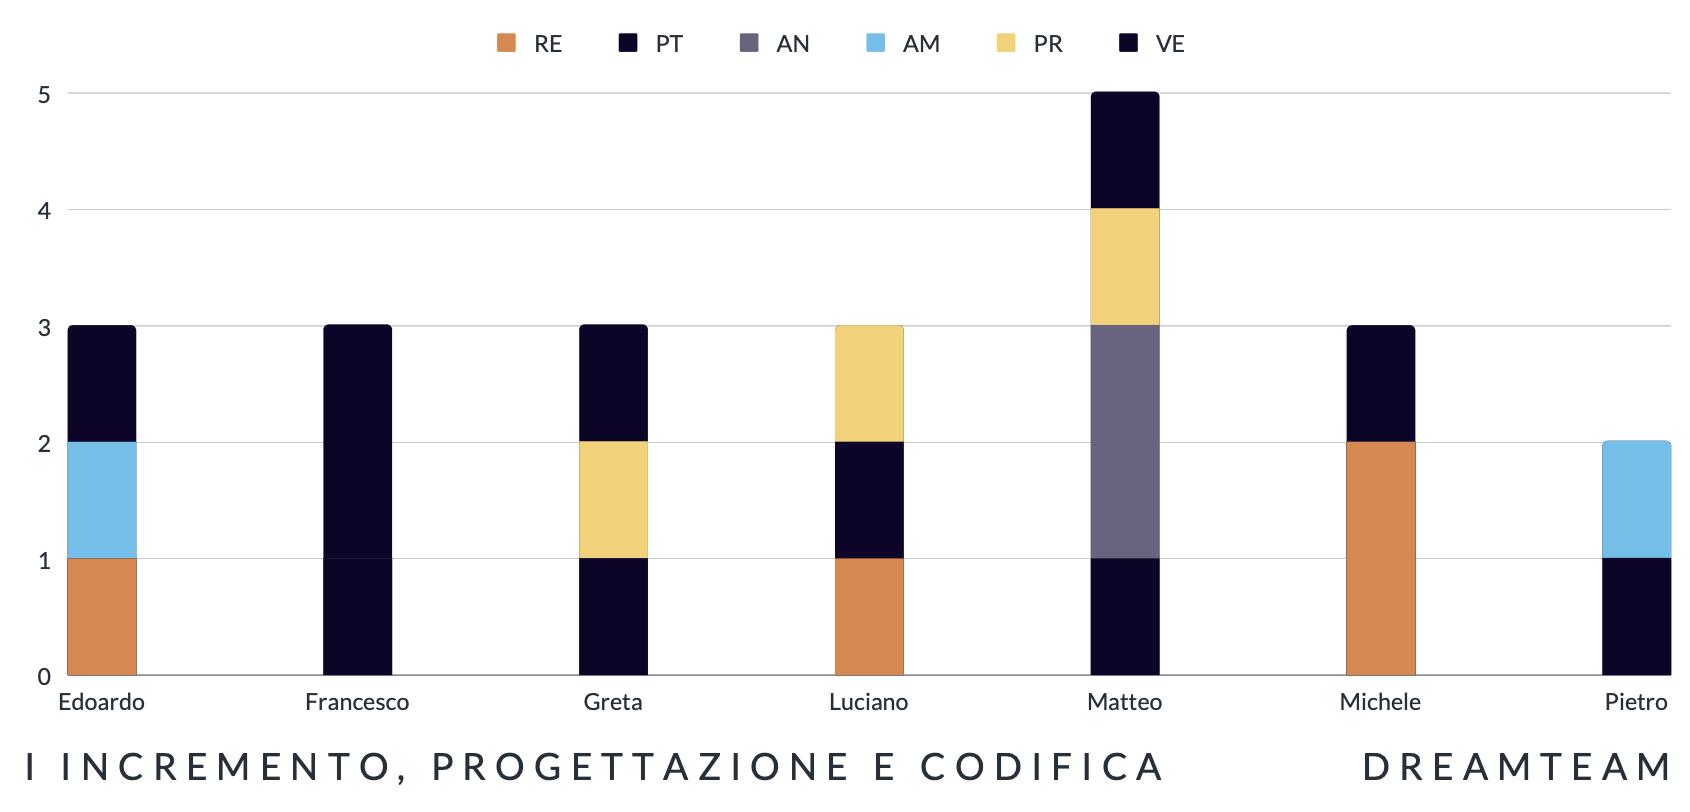
\includegraphics[scale=0.55]{Sezioni/SezioniPreventivo/grafici/Preventivo_progettazione_I.png}
\caption{Istogramma della ripartizione delle ore nel I incremento di Progettazione e Codifica}
\end{figure}

\subsubsubsection{Prospetto economico}
La seguente tabella rappresenta le ore totali dedicate ad ogni ruolo e il costo in euro:

\begin{table}[H]
\begin{center}
\rowcolors{2}{gray!25}{white}
\renewcommand{\arraystretch}{1.5}
\begin{tabular}{ m{0.3\textwidth}<{\centering}  m{0.2\textwidth}<{\centering} m{0.2\textwidth}<{\centering}}
	\rowcolor{darkblue}
	\textcolor{white}{\textbf{Ruolo}}&\textcolor{white}{\textbf{Totale ore}}&\textcolor{white}{\textbf{Costo totale (\euro)}}\\ 

	Responsabile  & 4 & 120 \\	
	
	Progettista & 5 & 100 \\
	
	Analista & 2 & 50 \\

	Amministratore & 2 & 50 \\
	
	Programmatore & 3 & 45 \\
	
	Verificatore & 6 & 90 \\
	
	\textbf{Totale} & 22 & 455 \\
	
\end{tabular}
\caption{Prospetto dei costi per ruolo nel I incremento di Progettazione e Codifica}
\end{center}
\end{table}

La tabella può essere rappresentata anche in forma visiva dal seguente aerogramma:
\begin{figure}[H]
\centering
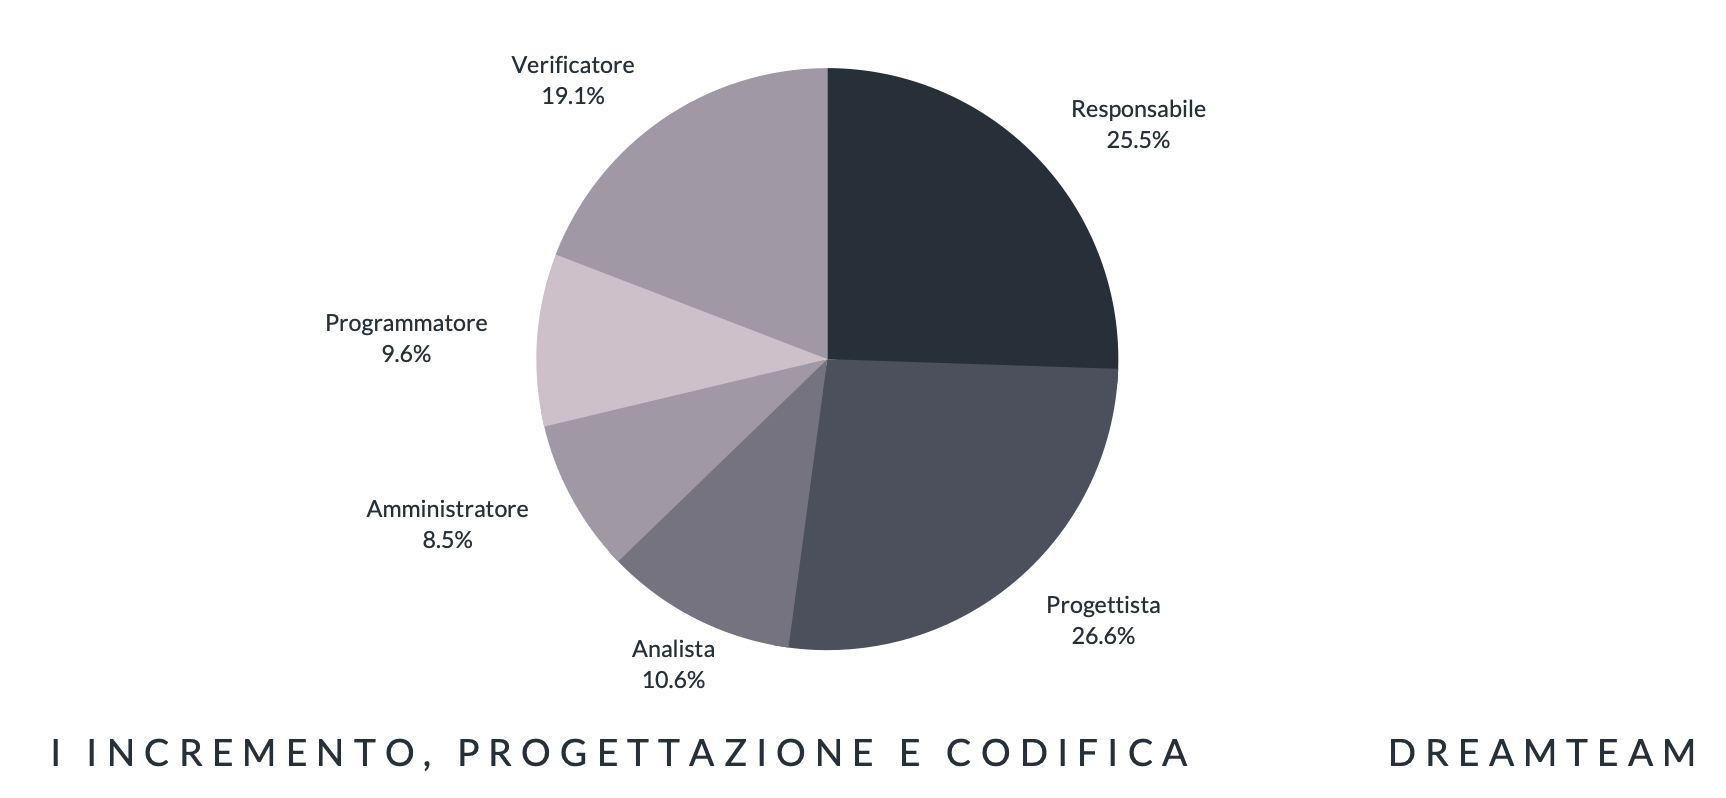
\includegraphics[scale=0.55]{Sezioni/SezioniPreventivo/grafici/Preventivo_torta_progettazione_I.png}
\caption{Grafico a torta della ripartizione per ruolo delle ore durante il I incremento di Progettazione e Codifica}
\end{figure}

\pagebreak

\subsubsection{II Incremento}
\subsubsubsection{Prospetto orario}
In questa incremento la distribuzione oraria è la seguente:
\begin{table}[H]
\begin{center}
\rowcolors{2}{gray!25}{white}
\renewcommand{\arraystretch}{1.25}
\begin{tabular}{ m{0.20\textwidth}<{\centering}  m{0.06\textwidth}<{\centering} m{0.06\textwidth}<{\centering} m{0.06\textwidth}<{\centering}  m{0.06\textwidth}<{\centering}  m{0.06\textwidth}<{\centering}  m{0.06\textwidth}<{\centering}  m{0.20\textwidth}<{\centering}   }
	\rowcolor{darkblue}
	\textcolor{white}{\textbf{Componente}} &\textcolor{white}{\textbf{Re}}&\textcolor{white}{\textbf{Pt}}&\textcolor{white}{\textbf{An}}&\textcolor{white}{\textbf{Am}}&\textcolor{white}{\textbf{Pr}}&\textcolor{white}{\textbf{Ve}}&\textcolor{white}{\textbf{Ore complessive}}\\ 
	Edoardo Pavan & 1 & 3 & 0 & 1 & 3 & 2 & 10 \\	
	
	Francesco Protopapa & 0 & 2 & 0 & 0 & 1 & 2 & 5 \\

	Greta Cavedon & 0 & 1 & 0 & 0 & 1 & 1 & 3 \\
	
	Luciano Wu & 1 & 1 & 0 & 1 & 1 & 0 & 4 \\
	
	Matteo Basso & 0 & 2 & 2 & 0 & 2 & 1 & 7 \\
	
	Michele Gatto & 1 & 1 & 0 & 0 & 1 & 1 & 4 \\
	
	Pietro Villatora & 0 & 2 & 0 & 0 & 5 & 1 & 8 \\
	
	\textbf{Ore totali ruolo} & 3 & 12 & 2 & 2 & 14 & 8 & 41 \\

\end{tabular}
\caption{Distribuzione oraria per ogni componente nel II incremento di Progettazione e Codifica}
\end{center}
\end{table}

La tabella può essere rappresentata anche in forma visiva dal seguente grafico:
\begin{figure}[H]
\centering
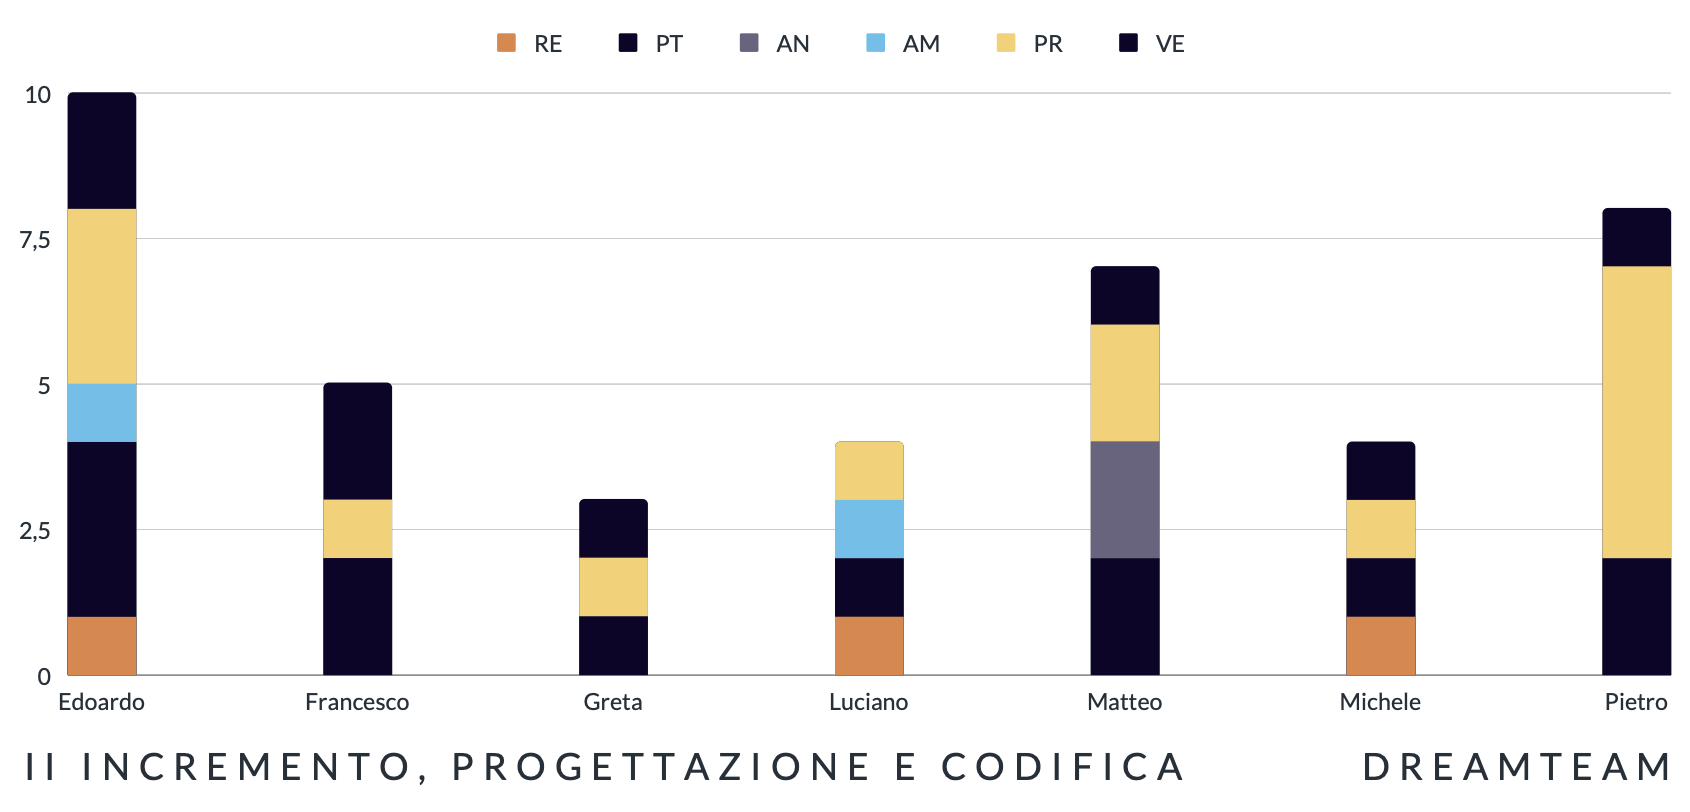
\includegraphics[scale=0.55]{Sezioni/SezioniPreventivo/grafici/Preventivo_progettazione_II.png}
\caption{Istogramma della ripartizione delle ore nel II incremento di Progettazione e Codifica}
\end{figure}

\subsubsubsection{Prospetto economico}
La seguente tabella rappresenta le ore totali dedicate ad ogni ruolo e il costo in euro:

\begin{table}[H]
\begin{center}
\rowcolors{2}{gray!25}{white}
\renewcommand{\arraystretch}{1.5}
\begin{tabular}{ m{0.3\textwidth}<{\centering}  m{0.2\textwidth}<{\centering} m{0.2\textwidth}<{\centering}}
	\rowcolor{darkblue}
	\textcolor{white}{\textbf{Ruolo}}&\textcolor{white}{\textbf{Totale ore}}&\textcolor{white}{\textbf{Costo totale (\euro)}}\\ 

	Responsabile  & 3 & 90 \\	
	
	Progettista & 12 & 240 \\
	
	Analista & 2 & 50 \\

	Amministratore & 2 & 50 \\
	
	Programmatore & 14 & 210 \\
	
	Verificatore & 8 & 120 \\
	
	\textbf{Totale} & 41 & 760 \\
	
\end{tabular}
\caption{Prospetto dei costi per ruolo nel II incremento di Progettazione e Codifica}
\end{center}
\end{table}

La tabella può essere rappresentata anche in forma visiva dal seguente aerogramma:
\begin{figure}[H]
\centering
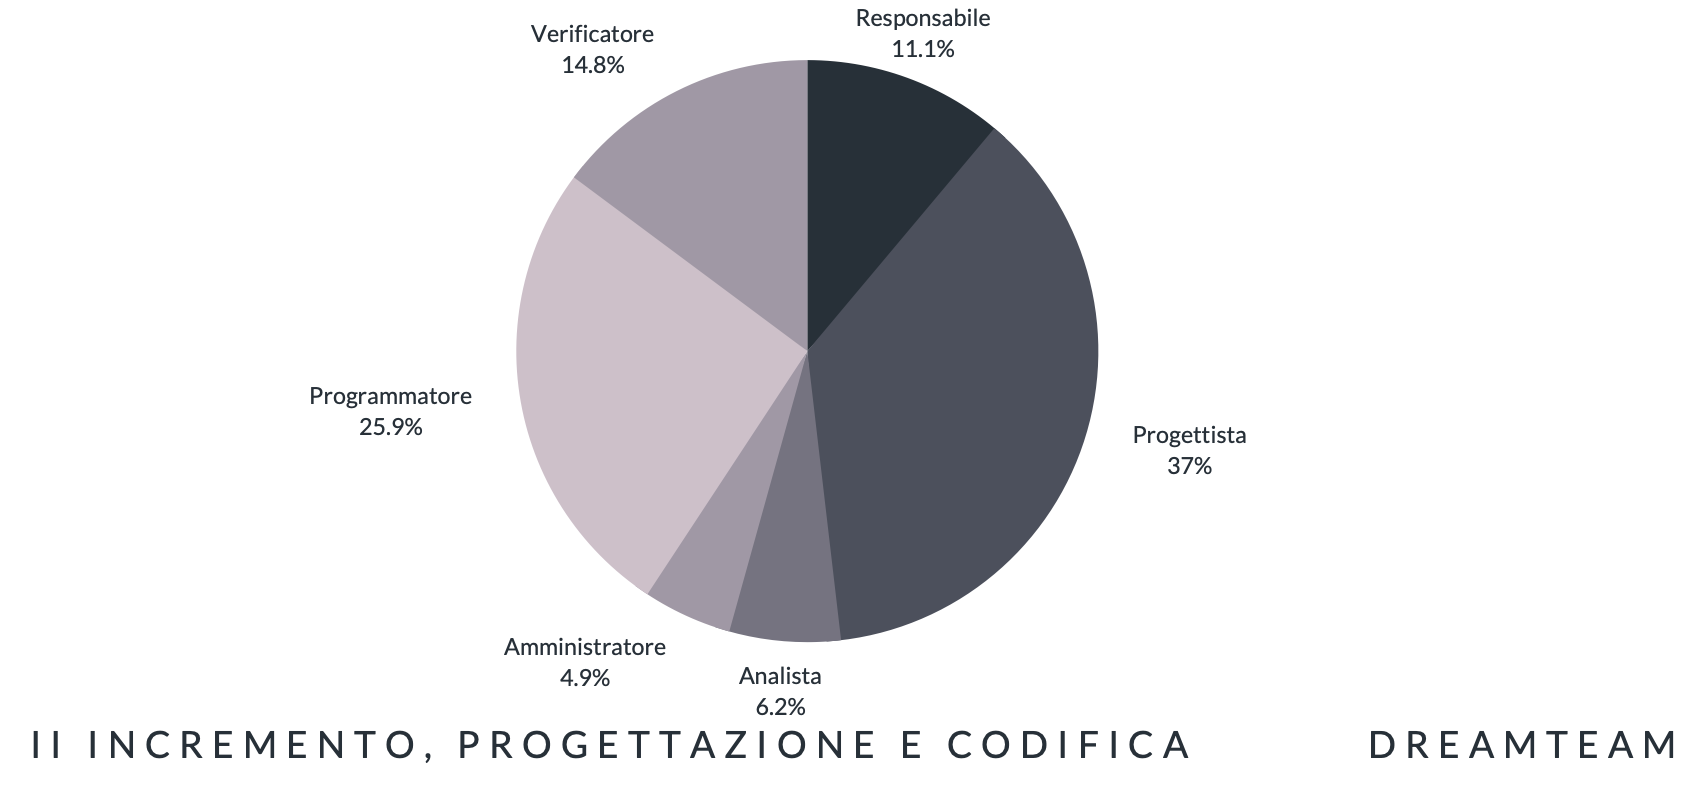
\includegraphics[scale=0.55]{Sezioni/SezioniPreventivo/grafici/Preventivo_torta_progettazione_II.png}
\caption{Grafico a torta della ripartizione per ruolo delle ore durante il II incremento di Progettazione e Codifica}
\end{figure}

\pagebreak


\subsubsection{III Incremento}
\subsubsubsection{Prospetto orario}
In questa fase la distribuzione oraria è la seguente:
\begin{table}[H]
\begin{center}
\rowcolors{2}{gray!25}{white}
\renewcommand{\arraystretch}{1.25}
\begin{tabular}{ m{0.20\textwidth}<{\centering}  m{0.06\textwidth}<{\centering} m{0.06\textwidth}<{\centering} m{0.06\textwidth}<{\centering}  m{0.06\textwidth}<{\centering}  m{0.06\textwidth}<{\centering}  m{0.06\textwidth}<{\centering}  m{0.20\textwidth}<{\centering}   }
	\rowcolor{darkblue}
	\textcolor{white}{\textbf{Componente}} &\textcolor{white}{\textbf{Re}}&\textcolor{white}{\textbf{Pt}}&\textcolor{white}{\textbf{An}}&\textcolor{white}{\textbf{Am}}&\textcolor{white}{\textbf{Pr}}&\textcolor{white}{\textbf{Ve}}&\textcolor{white}{\textbf{Ore complessive}}\\ 
	Edoardo Pavan & 0 & 2 & 0 & 1 & 3 & 1 & 7 \\	
	
	Francesco Protopapa & 1 & 1 & 0 & 0 & 3 & 0 & 5 \\

	Greta Cavedon & 1 & 1 & 0 & 0 & 3 & 1 & 6 \\
	
	Luciano Wu & 0 & 1 & 0 & 0 & 3 & 1 & 5 \\
	
	Matteo Basso & 0 & 2 & 1 & 0 & 2 & 1 & 6 \\
	
	Michele Gatto & 0 & 2 & 0 & 0 & 4 & 2 & 8 \\
	
	Pietro Villatora & 0 & 1 & 0 & 0 & 5 & 1 & 7 \\
	
	\textbf{Ore totali ruolo} & 2 & 10 & 1 & 1 & 23 & 7 & 44 \\

\end{tabular}
\caption{Distribuzione oraria per ogni componente nel III incremento di Progettazione e Codifica}
\end{center}
\end{table}

La tabella può essere rappresentata anche in forma visiva dal seguente grafico:
\begin{figure}[H]
\centering
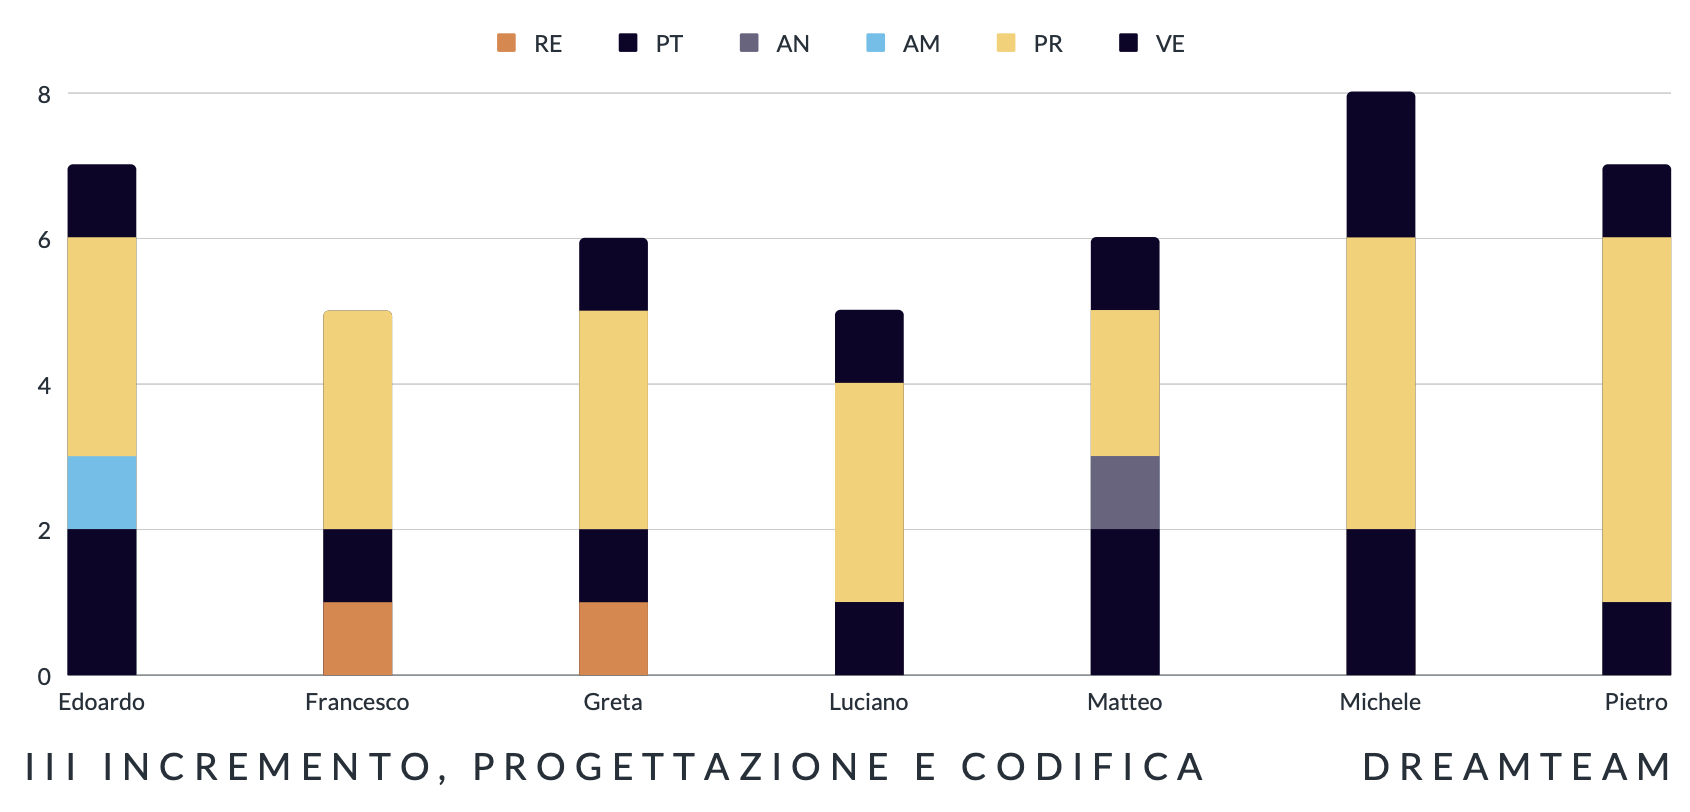
\includegraphics[scale=0.55]{Sezioni/SezioniPreventivo/grafici/Preventivo_progettazione_III.png}
\caption{Istogramma della ripartizione delle ore nel III incremento di Progettazione e Codifica}
\end{figure}

\subsubsubsection{Prospetto economico}
La seguente tabella rappresenta le ore totali dedicate ad ogni ruolo e il costo in euro:

\begin{table}[H]
\begin{center}
\rowcolors{2}{gray!25}{white}
\renewcommand{\arraystretch}{1.5}
\begin{tabular}{ m{0.3\textwidth}<{\centering}  m{0.2\textwidth}<{\centering} m{0.2\textwidth}<{\centering}}
	\rowcolor{darkblue}
	\textcolor{white}{\textbf{Ruolo}}&\textcolor{white}{\textbf{Totale ore}}&\textcolor{white}{\textbf{Costo totale (\euro)}}\\ 

	Responsabile  & 2 & 60 \\	
	
	Progettista & 10 & 200 \\
	
	Analista & 1 & 25 \\

	Amministratore & 1 & 25 \\
	
	Programmatore & 23 & 345 \\
	
	Verificatore & 7 & 105 \\
	
	\textbf{Totale} & 44 & 760 \\
	
\end{tabular}
\caption{Prospetto dei costi per ruolo nel III incremento di Progettazione e Codifica}
\end{center}
\end{table}

La tabella può essere rappresentata anche in forma visiva dal seguente aerogramma:
\begin{figure}[H]
\centering
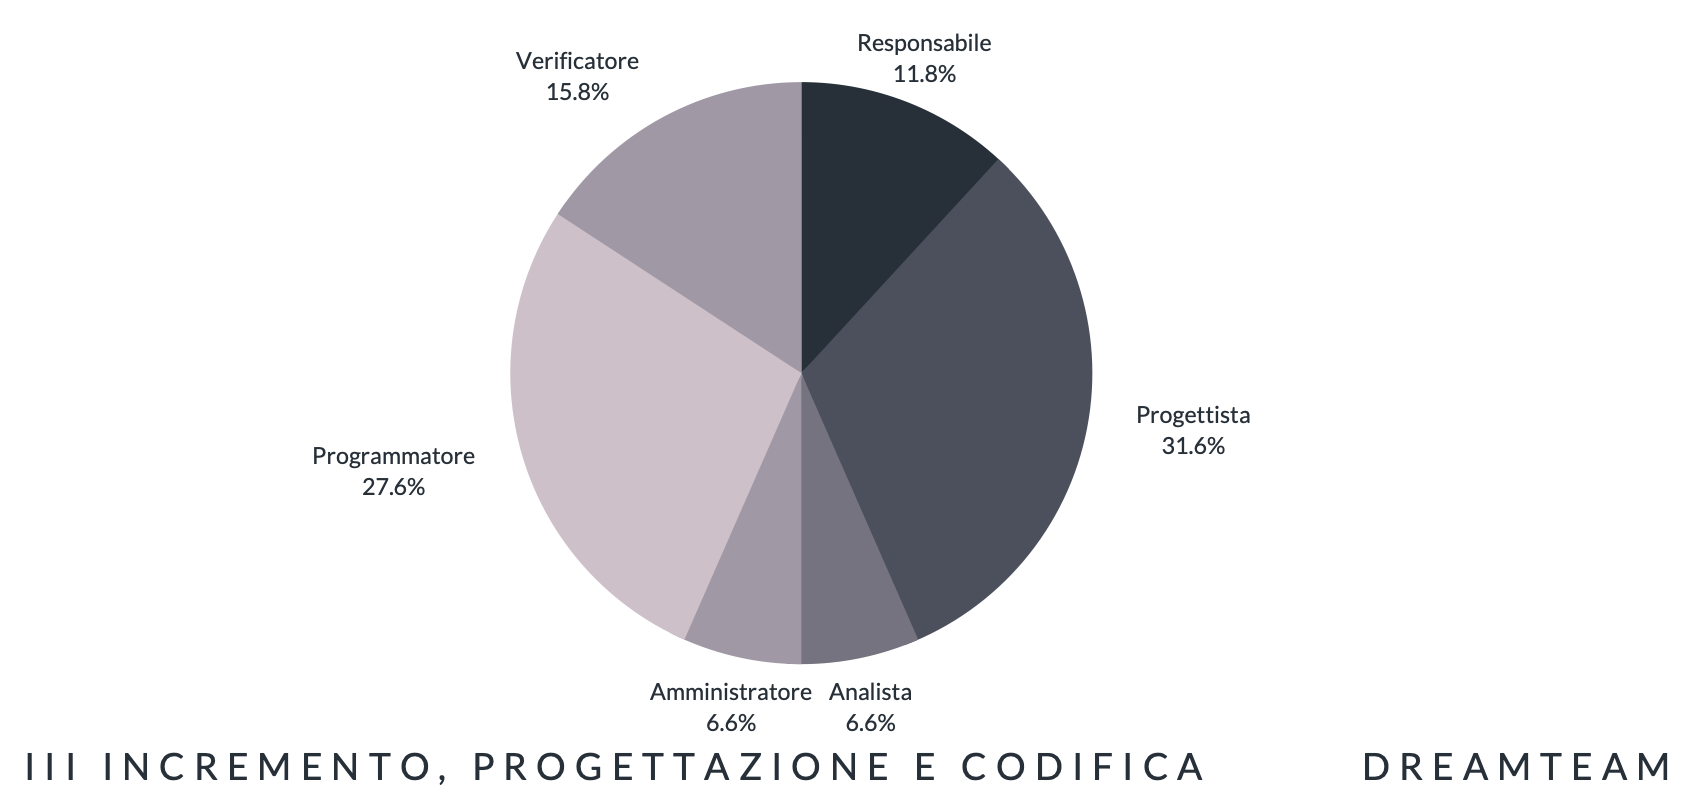
\includegraphics[scale=0.55]{Sezioni/SezioniPreventivo/grafici/Preventivo_torta_progettazione_III.png}
\caption{Grafico a torta della ripartizione per ruolo delle ore durante il III incremento di Progettazione e Codifica}
\end{figure}

\pagebreak


\subsubsection{IV Incremento}
\subsubsubsection{Prospetto orario}
In questa fase la distribuzione oraria è la seguente:
\begin{table}[H]
\begin{center}
\rowcolors{2}{gray!25}{white}
\renewcommand{\arraystretch}{1.25}
\begin{tabular}{ m{0.20\textwidth}<{\centering}  m{0.06\textwidth}<{\centering} m{0.06\textwidth}<{\centering} m{0.06\textwidth}<{\centering}  m{0.06\textwidth}<{\centering}  m{0.06\textwidth}<{\centering}  m{0.06\textwidth}<{\centering}  m{0.20\textwidth}<{\centering}   }
	\rowcolor{darkblue}
	\textcolor{white}{\textbf{Componente}} &\textcolor{white}{\textbf{Re}}&\textcolor{white}{\textbf{Pt}}&\textcolor{white}{\textbf{An}}&\textcolor{white}{\textbf{Am}}&\textcolor{white}{\textbf{Pr}}&\textcolor{white}{\textbf{Ve}}&\textcolor{white}{\textbf{Ore complessive}}\\ 
	Edoardo Pavan & 0 & 2 & 0 & 1 & 3 & 1 & 7 \\	
	
	Francesco Protopapa & 1 & 1 & 0 & 0 & 4 & 0 & 6 \\

	Greta Cavedon & 1 & 1 & 0 & 0 & 3 & 1 & 6 \\
	
	Luciano Wu & 0 & 2 & 0 & 1 & 3 & 1 & 7 \\
	
	Matteo Basso & 0 & 1 & 1 & 0 & 2 & 1 & 5 \\
	
	Michele Gatto & 0 & 1 & 0 & 0 & 4 & 1 & 6 \\
	
	Pietro Villatora & 0 & 1 & 0 & 0 & 5 & 1 & 7 \\
	
	\textbf{Ore totali ruolo} & 2 & 9 & 1 & 2 & 24 & 6 & 44 \\

\end{tabular}
\caption{Distribuzione oraria per ogni componente nel IV incremento di Progettazione e Codifica}
\end{center}
\end{table}

La tabella può essere rappresentata anche in forma visiva dal seguente grafico:
\begin{figure}[H]
\centering
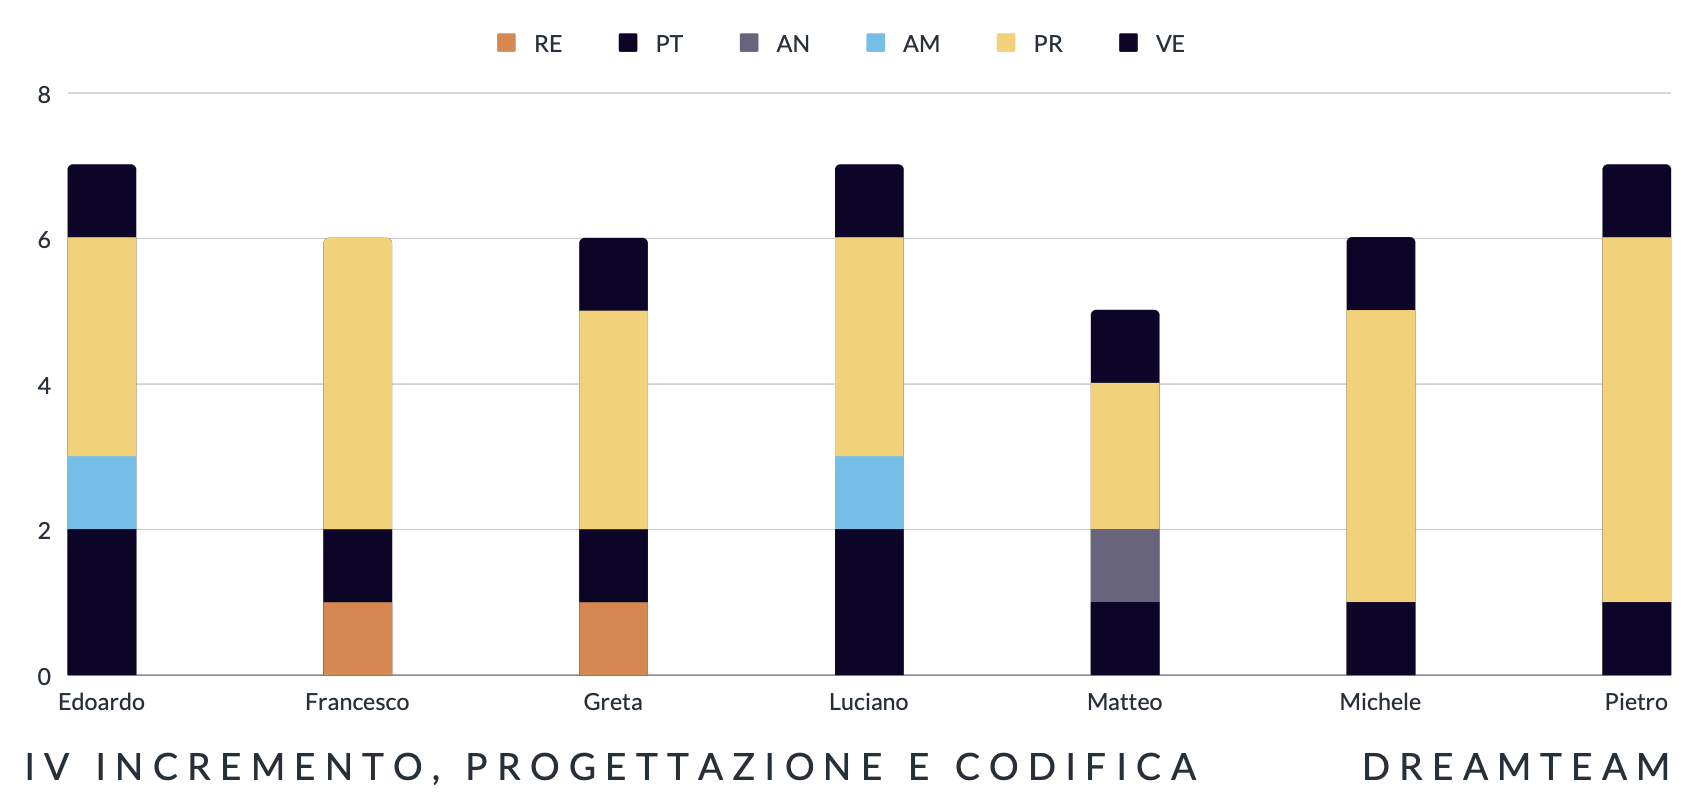
\includegraphics[scale=0.55]{Sezioni/SezioniPreventivo/grafici/Preventivo_progettazione_IV.png}
\caption{Istogramma della ripartizione delle ore nel IV incremento di Progettazione e Codifica}
\end{figure}

\subsubsubsection{Prospetto economico}
La seguente tabella rappresenta le ore totali dedicate ad ogni ruolo e il costo in euro:

\begin{table}[H]
\begin{center}
\rowcolors{2}{gray!25}{white}
\renewcommand{\arraystretch}{1.5}
\begin{tabular}{ m{0.3\textwidth}<{\centering}  m{0.2\textwidth}<{\centering} m{0.2\textwidth}<{\centering}}
	\rowcolor{darkblue}
	\textcolor{white}{\textbf{Ruolo}}&\textcolor{white}{\textbf{Totale ore}}&\textcolor{white}{\textbf{Costo totale (\euro)}}\\ 

	Responsabile  & 2 & 60 \\	
	
	Progettista & 9 & 225 \\
	
	Analista & 1 & 25 \\

	Amministratore & 2 & 50 \\
	
	Programmatore & 24 & 360 \\
	
	Verificatore & 6 & 90 \\
	
	\textbf{Totale} & 44 & 810 \\
	
\end{tabular}
\caption{Prospetto dei costi per ruolo nel IV incremento di Progettazione e Codifica}
\end{center}
\end{table}

La tabella può essere rappresentata anche in forma visiva dal seguente aerogramma:
\begin{figure}[H]
\centering
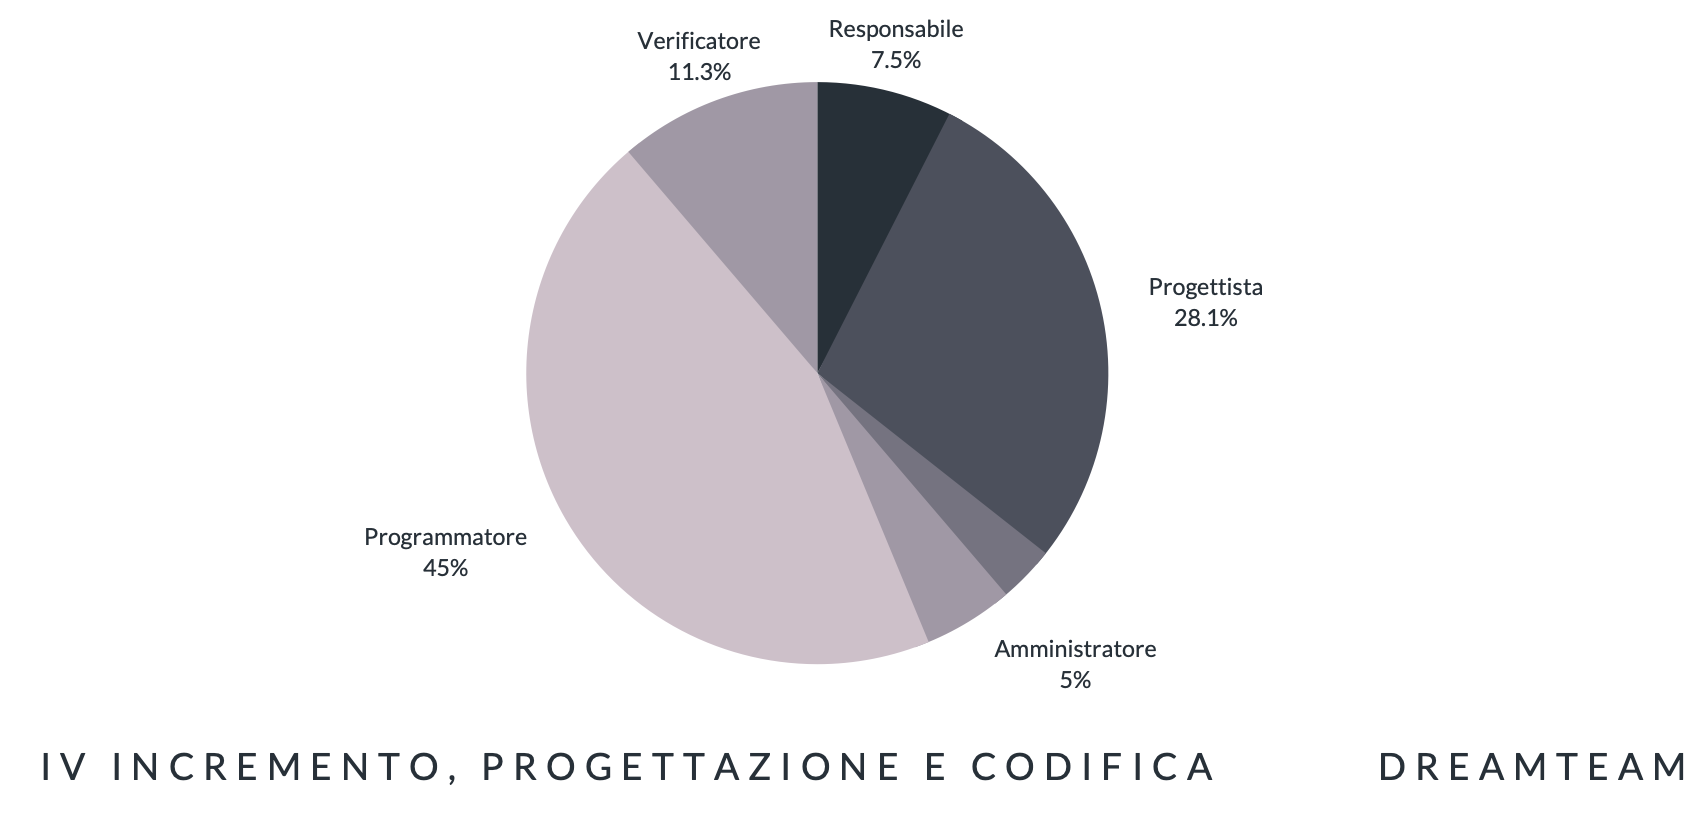
\includegraphics[scale=0.55]{Sezioni/SezioniPreventivo/grafici/Preventivo_torta_progettazione_IV.png}
\caption{Grafico a torta della ripartizione per ruolo delle ore durante il IV incremento di Progettazione e Codifica}
\end{figure}

\pagebreak

\subsubsection{V Incremento}
\subsubsubsection{Prospetto orario}
In questa fase la distribuzione oraria è la seguente:
\begin{table}[H]
\begin{center}
\rowcolors{2}{gray!25}{white}
\renewcommand{\arraystretch}{1.25}
\begin{tabular}{ m{0.20\textwidth}<{\centering}  m{0.06\textwidth}<{\centering} m{0.06\textwidth}<{\centering} m{0.06\textwidth}<{\centering}  m{0.06\textwidth}<{\centering}  m{0.06\textwidth}<{\centering}  m{0.06\textwidth}<{\centering}  m{0.20\textwidth}<{\centering}   }
	\rowcolor{darkblue}
	\textcolor{white}{\textbf{Componente}} &\textcolor{white}{\textbf{Re}}&\textcolor{white}{\textbf{Pt}}&\textcolor{white}{\textbf{An}}&\textcolor{white}{\textbf{Am}}&\textcolor{white}{\textbf{Pr}}&\textcolor{white}{\textbf{Ve}}&\textcolor{white}{\textbf{Ore complessive}}\\ 
	Edoardo Pavan & 0 & 2 & 0 & 1 & 3 & 1 & 7 \\	
	
	Francesco Protopapa & 0 & 1 & 0 & 0 & 4 & 1 & 6 \\

	Greta Cavedon & 0 & 0 & 0 & 0 & 2 & 1 & 3 \\
	
	Luciano Wu & 1 & 2 & 0 & 0 & 2 & 2 & 7 \\
	
	Matteo Basso & 0 & 1 & 1 & 0 & 2 & 1 & 5 \\
	
	Michele Gatto & 1 & 1 & 0 & 0 & 3 & 0 & 5 \\
	
	Pietro Villatora & 0 & 1 & 0 & 1 & 5 & 0 & 7 \\
	
	\textbf{Ore totali ruolo} & 2 & 8 & 1 & 2 & 21 & 6 & 40 \\

\end{tabular}
\caption{Distribuzione oraria per ogni componente nel V incremento di Progettazione e Codifica}
\end{center}
\end{table}

La tabella può essere rappresentata anche in forma visiva dal seguente grafico:
\begin{figure}[H]
\centering
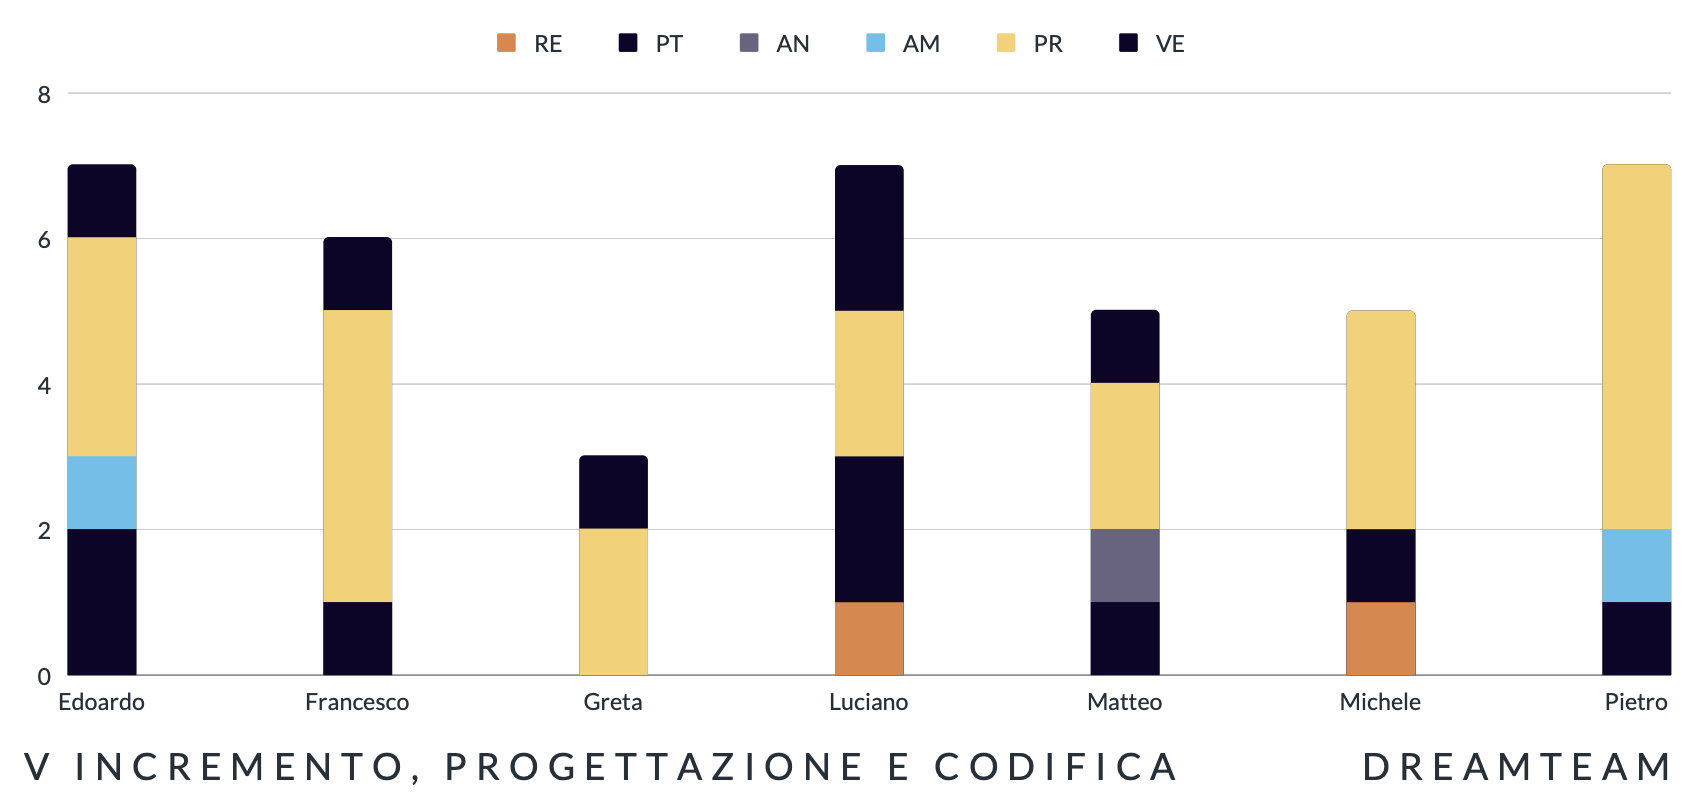
\includegraphics[scale=0.55]{Sezioni/SezioniPreventivo/grafici/Preventivo_progettazione_V.png}
\caption{Istogramma della ripartizione delle ore nel V incremento di Progettazione e Codifica}
\end{figure}

\subsubsubsection{Prospetto economico}
La seguente tabella rappresenta le ore totali dedicate ad ogni ruolo e il costo in euro:

\begin{table}[H]
\begin{center}
\rowcolors{2}{gray!25}{white}
\renewcommand{\arraystretch}{1.5}
\begin{tabular}{ m{0.3\textwidth}<{\centering}  m{0.2\textwidth}<{\centering} m{0.2\textwidth}<{\centering}}
	\rowcolor{darkblue}
	\textcolor{white}{\textbf{Ruolo}}&\textcolor{white}{\textbf{Totale ore}}&\textcolor{white}{\textbf{Costo totale (\euro)}}\\ 

	Responsabile  & 2 & 60 \\	
	
	Progettista & 8 & 160 \\
	
	Analista & 1 & 25 \\

	Amministratore & 2 & 50 \\
	
	Programmatore & 21 & 315 \\
	
	Verificatore & 6 & 90 \\
	
	\textbf{Totale} & 40 & 700 \\
	
\end{tabular}
\caption{Prospetto dei costi per ruolo nel V incremento di Progettazione e Codifica}
\end{center}
\end{table}

La tabella può essere rappresentata anche in forma visiva dal seguente aerogramma:
\begin{figure}[H]
\centering
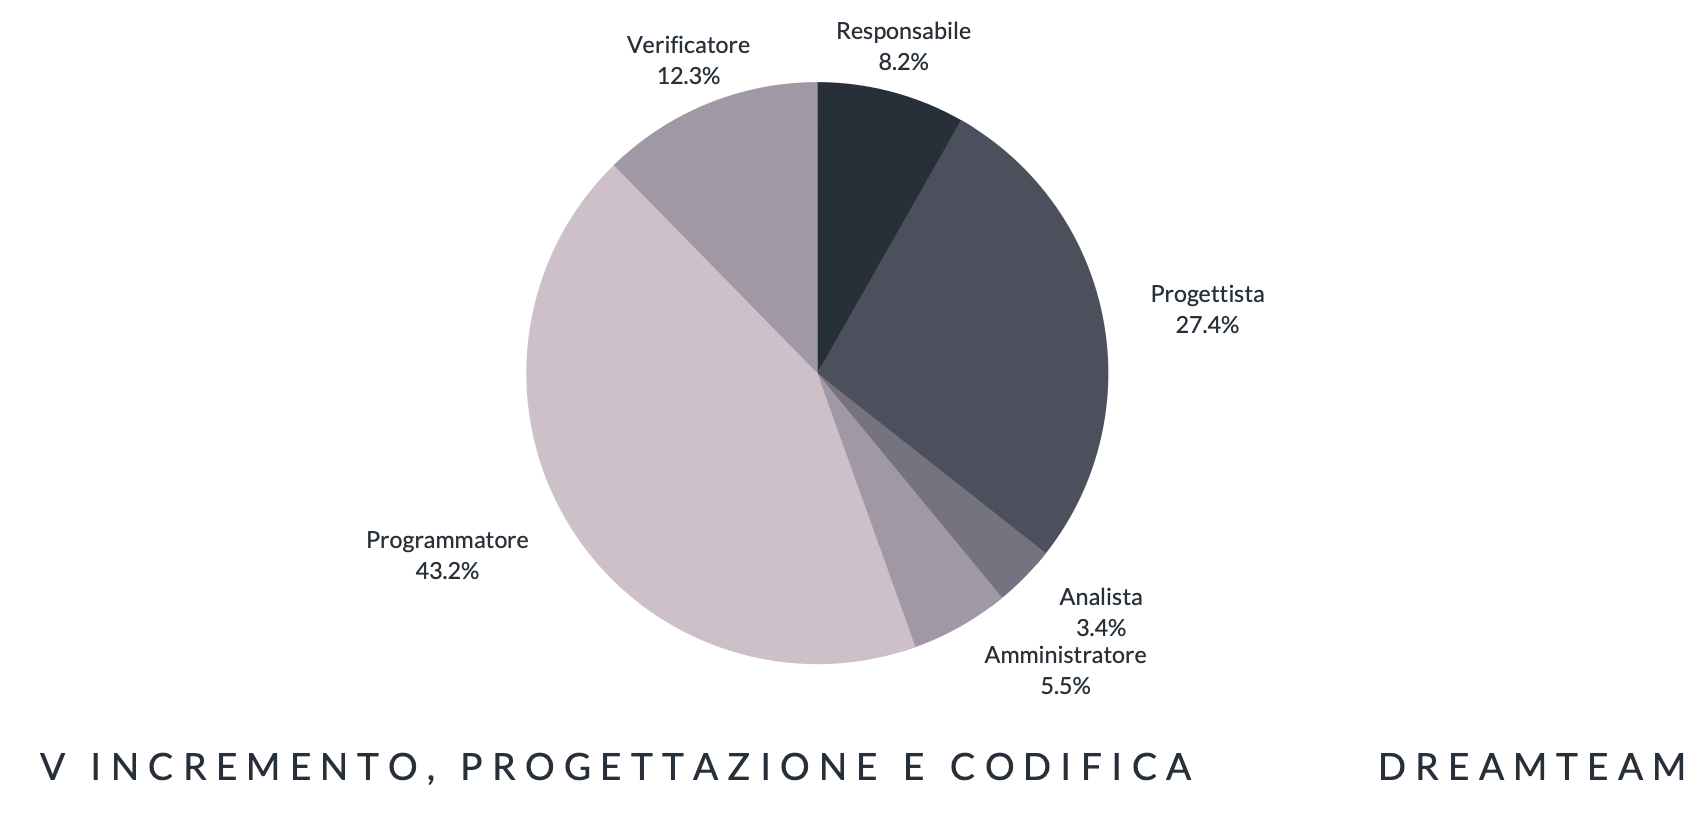
\includegraphics[scale=0.55]{Sezioni/SezioniPreventivo/grafici/Preventivo_torta_progettazione_V.png}
\caption{Grafico a torta della ripartizione per ruolo delle ore durante il V incremento di Progettazione e Codifica}
\end{figure}

\pagebreak


\subsubsection{VI Incremento}
\subsubsubsection{Prospetto orario}
In questa fase la distribuzione oraria è la seguente:
\begin{table}[H]
\begin{center}
\rowcolors{2}{gray!25}{white}
\renewcommand{\arraystretch}{1.25}
\begin{tabular}{ m{0.20\textwidth}<{\centering}  m{0.06\textwidth}<{\centering} m{0.06\textwidth}<{\centering} m{0.06\textwidth}<{\centering}  m{0.06\textwidth}<{\centering}  m{0.06\textwidth}<{\centering}  m{0.06\textwidth}<{\centering}  m{0.20\textwidth}<{\centering}   }
	\rowcolor{darkblue}
	\textcolor{white}{\textbf{Componente}} &\textcolor{white}{\textbf{Re}}&\textcolor{white}{\textbf{Pt}}&\textcolor{white}{\textbf{An}}&\textcolor{white}{\textbf{Am}}&\textcolor{white}{\textbf{Pr}}&\textcolor{white}{\textbf{Ve}}&\textcolor{white}{\textbf{Ore complessive}}\\ 
	Edoardo Pavan & 0 & 2 & 0 & 1 & 3 & 1 & 7 \\	
	
	Francesco Protopapa & 0 & 0 & 0 & 1 & 4 & 0 & 5 \\

	Greta Cavedon & 0 & 1 & 0 & 0 & 2 & 2 & 5 \\
	
	Luciano Wu & 1 & 1 & 0 & 0 & 2 & 1 & 5 \\
	
	Matteo Basso & 0 & 1 & 1 & 0 & 2 & 1 & 5 \\
	
	Michele Gatto & 1 & 2 & 0 & 0 & 3 & 1 & 6 \\
	
	Pietro Villatora & 0 & 1 & 0 & 0 & 5 & 1 & 7 \\
	
	\textbf{Ore totali ruolo} & 2 & 8 & 1 & 2 & 21 & 6 & 40 \\

\end{tabular}
\caption{Distribuzione oraria per ogni componente nel VI incremento di Progettazione e Codifica}
\end{center}
\end{table}

La tabella può essere rappresentata anche in forma visiva dal seguente grafico:
\begin{figure}[H]
\centering
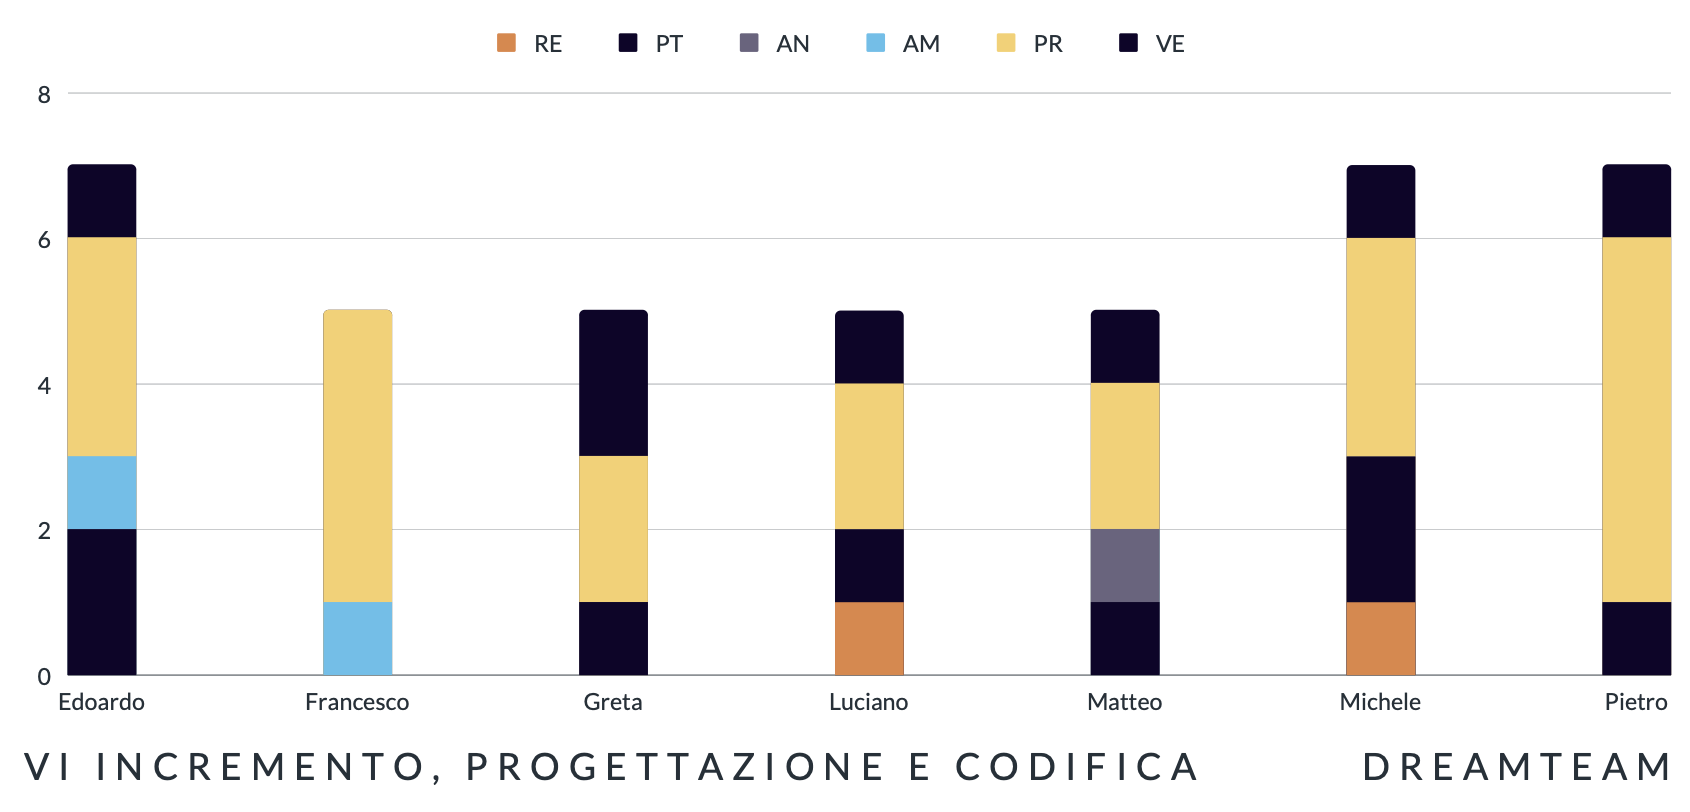
\includegraphics[scale=0.55]{Sezioni/SezioniPreventivo/grafici/Preventivo_progettazione_VI.png}
\caption{Istogramma della ripartizione delle ore nel VI incremento di Progettazione e Codifica}
\end{figure}

\subsubsubsection{Prospetto economico}
La seguente tabella rappresenta le ore totali dedicate ad ogni ruolo e il costo in euro:

\begin{table}[H]
\begin{center}
\rowcolors{2}{gray!25}{white}
\renewcommand{\arraystretch}{1.5}
\begin{tabular}{ m{0.3\textwidth}<{\centering}  m{0.2\textwidth}<{\centering} m{0.2\textwidth}<{\centering}}
	\rowcolor{darkblue}
	\textcolor{white}{\textbf{Ruolo}}&\textcolor{white}{\textbf{Totale ore}}&\textcolor{white}{\textbf{Costo totale (\euro)}}\\ 

	Responsabile  & 2 & 60 \\	
	
	Progettista & 8 & 160 \\
	
	Analista & 1 & 25 \\

	Amministratore & 2 & 50 \\
	
	Programmatore & 21 & 315 \\
	
	Verificatore & 6 & 90 \\
	
	\textbf{Totale} & 40 & 700 \\
	
\end{tabular}
\caption{Prospetto dei costi per ruolo nel VI incremento di Progettazione e Codifica}
\end{center}
\end{table}

La tabella può essere rappresentata anche in forma visiva dal seguente aerogramma:
\begin{figure}[H]
\centering
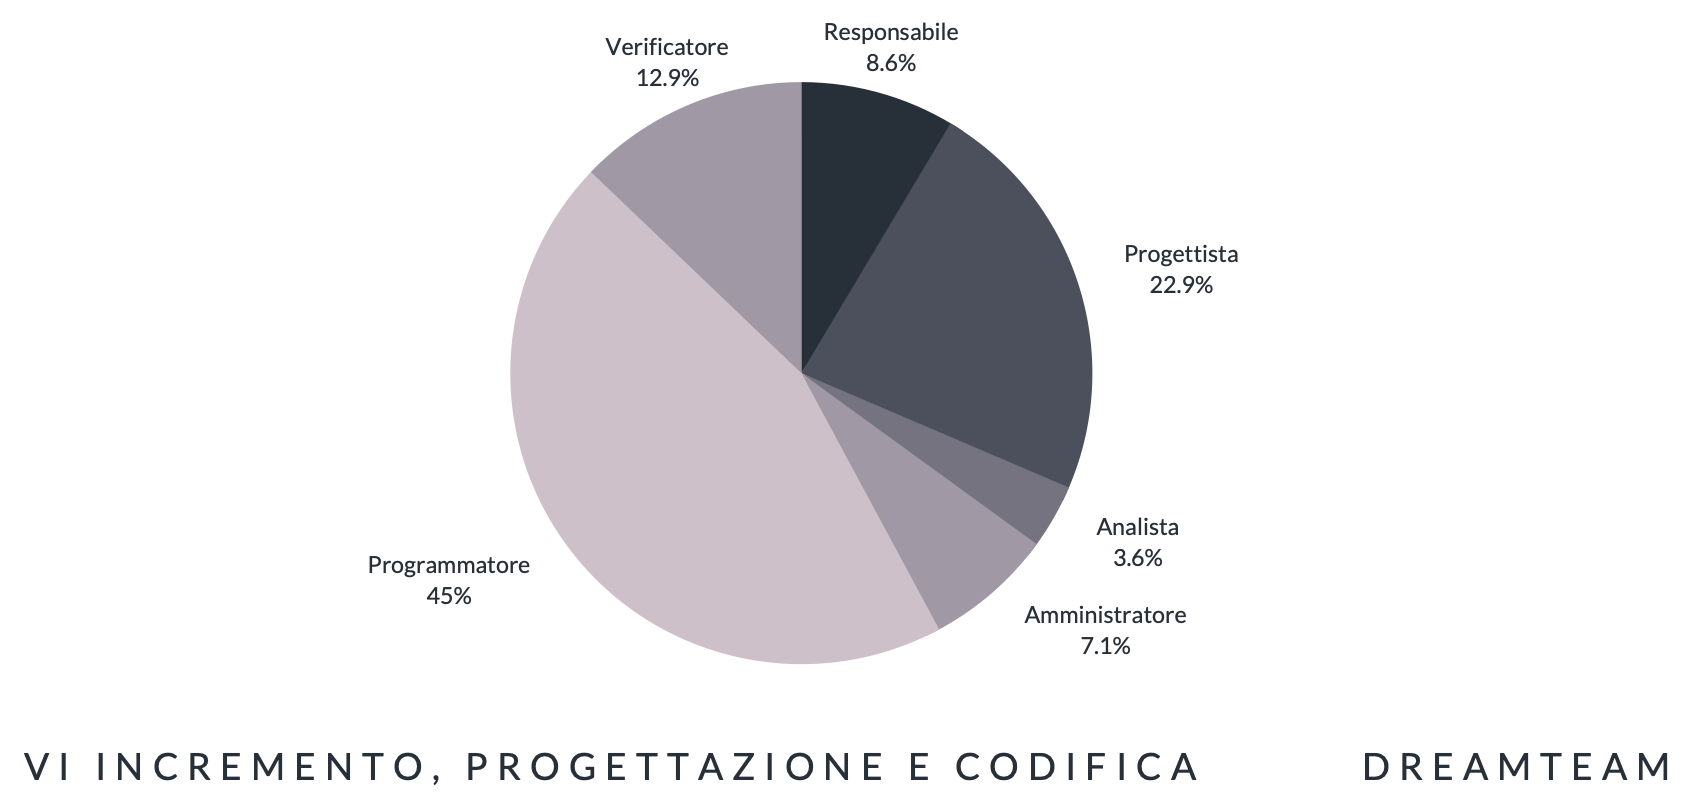
\includegraphics[scale=0.55]{Sezioni/SezioniPreventivo/grafici/Preventivo_torta_progettazione_VI.png}
\caption{Grafico a torta della ripartizione per ruolo delle ore durante il VI incremento di Progettazione e Codifica}
\end{figure}

\pagebreak


\subsubsection{VII Incremento}
\subsubsubsection{Prospetto orario}
In questa fase la distribuzione oraria è la seguente:
\begin{table}[H]
\begin{center}
\rowcolors{2}{gray!25}{white}
\renewcommand{\arraystretch}{1.25}
\begin{tabular}{ m{0.20\textwidth}<{\centering}  m{0.06\textwidth}<{\centering} m{0.06\textwidth}<{\centering} m{0.06\textwidth}<{\centering}  m{0.06\textwidth}<{\centering}  m{0.06\textwidth}<{\centering}  m{0.06\textwidth}<{\centering}  m{0.20\textwidth}<{\centering}   }
	\rowcolor{darkblue}
	\textcolor{white}{\textbf{Componente}} &\textcolor{white}{\textbf{Re}}&\textcolor{white}{\textbf{Pt}}&\textcolor{white}{\textbf{An}}&\textcolor{white}{\textbf{Am}}&\textcolor{white}{\textbf{Pr}}&\textcolor{white}{\textbf{Ve}}&\textcolor{white}{\textbf{Ore complessive}}\\ 
	Edoardo Pavan & 0 & 2 & 0 & 1 & 3 & 1 & 7 \\	
	
	Francesco Protopapa & 0 & 1 & 0 & 0 & 2 & 0 & 3 \\

	Greta Cavedon & 1 & 1 & 0 & 0 & 2 & 1 & 5 \\
	
	Luciano Wu & 0 & 1 & 0 & 1 & 2 & 1 & 5 \\
	
	Matteo Basso & 0 & 0 & 1 & 0 & 2 & 1 & 4 \\
	
	Michele Gatto & 0 & 1 & 0 & 0 & 3 & 0 & 4 \\
	
	Pietro Villatora & 0 & 0 & 0 & 0 & 5 & 1 & 6 \\
	
	\textbf{Ore totali ruolo} & 1 & 6 & 1 & 2 & 19 & 5 & 34 \\

\end{tabular}
\caption{Distribuzione oraria per ogni componente nel VII incremento di Progettazione e Codifica}
\end{center}
\end{table}

La tabella può essere rappresentata anche in forma visiva dal seguente grafico:
\begin{figure}[H]
\centering
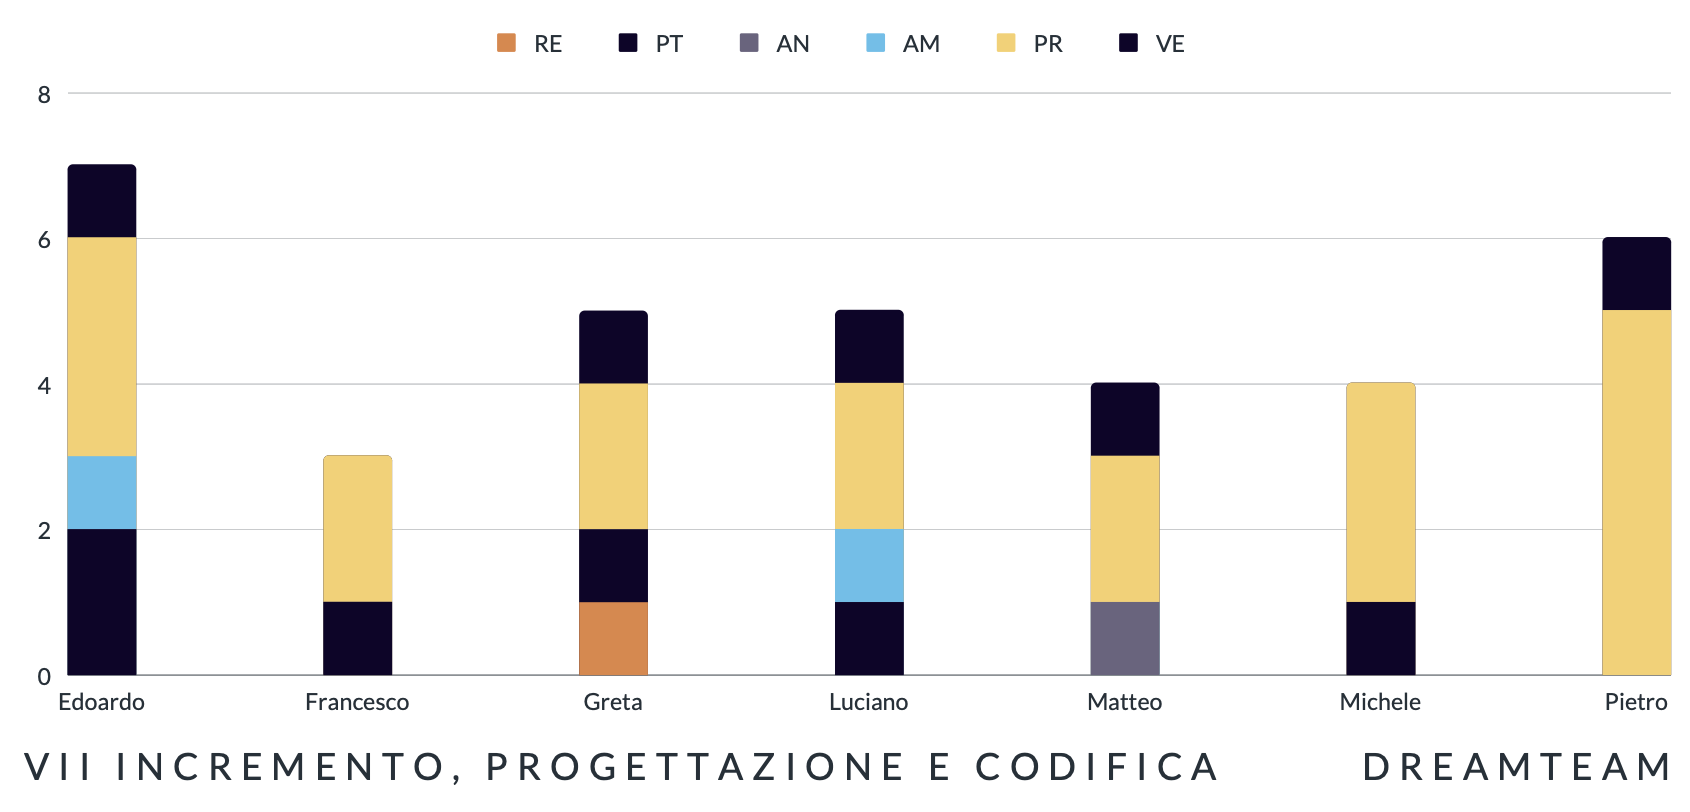
\includegraphics[scale=0.55]{Sezioni/SezioniPreventivo/grafici/Preventivo_progettazione_VII.png}
\caption{Istogramma della ripartizione delle ore nel VII incremento di Progettazione e Codifica}
\end{figure}

\subsubsubsection{Prospetto economico}
La seguente tabella rappresenta le ore totali dedicate ad ogni ruolo e il costo in euro:

\begin{table}[H]
\begin{center}
\rowcolors{2}{gray!25}{white}
\renewcommand{\arraystretch}{1.5}
\begin{tabular}{ m{0.3\textwidth}<{\centering}  m{0.2\textwidth}<{\centering} m{0.2\textwidth}<{\centering}}
	\rowcolor{darkblue}
	\textcolor{white}{\textbf{Ruolo}}&\textcolor{white}{\textbf{Totale ore}}&\textcolor{white}{\textbf{Costo totale (\euro)}}\\ 

	Responsabile  & 1 & 30 \\	
	
	Progettista & 6 & 120 \\
	
	Analista & 1 & 25 \\

	Amministratore & 2 & 50 \\
	
	Programmatore & 19 & 285 \\
	
	Verificatore & 5 & 75 \\
	
	\textbf{Totale} & 34 & 585 \\
	
\end{tabular}
\caption{Prospetto dei costi per ruolo nel VII incremento di Progettazione e Codifica}
\end{center}
\end{table}

La tabella può essere rappresentata anche in forma visiva dal seguente aerogramma:
\begin{figure}[H]
\centering
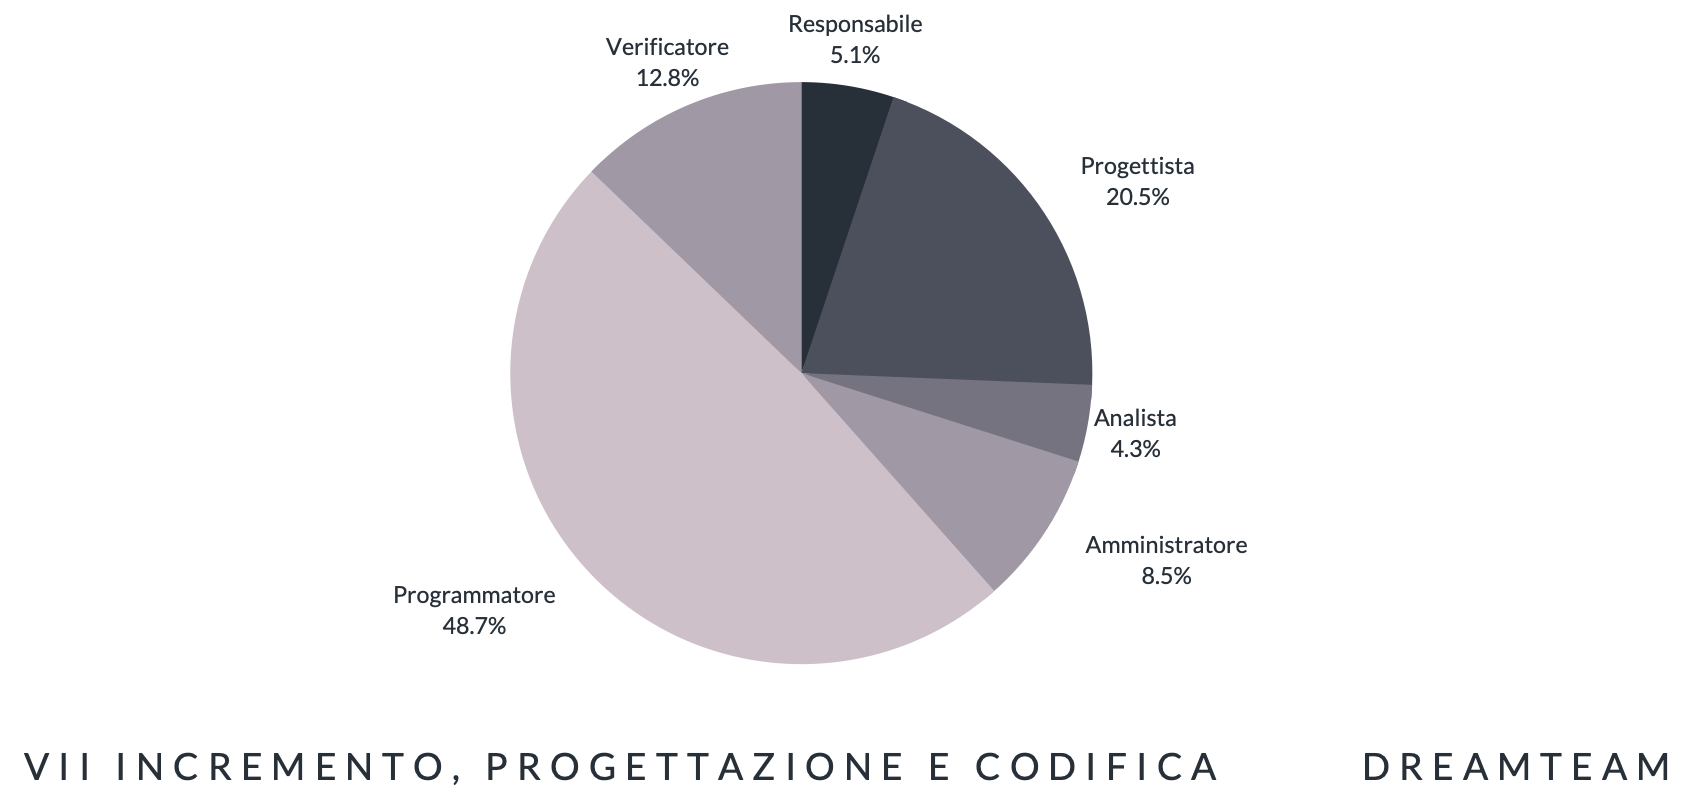
\includegraphics[scale=0.55]{Sezioni/SezioniPreventivo/grafici/Preventivo_torta_progettazione_VII.png}
\caption{Grafico a torta della ripartizione per ruolo delle ore durante il VII incremento di Progettazione e Codifica}
\end{figure}

\pagebreak


\subsubsection{VIII Incremento}
\subsubsubsection{Prospetto orario}
In questa fase la distribuzione oraria è la seguente:
\begin{table}[H]
\begin{center}
\rowcolors{2}{gray!25}{white}
\renewcommand{\arraystretch}{1.25}
\begin{tabular}{ m{0.20\textwidth}<{\centering}  m{0.06\textwidth}<{\centering} m{0.06\textwidth}<{\centering} m{0.06\textwidth}<{\centering}  m{0.06\textwidth}<{\centering}  m{0.06\textwidth}<{\centering}  m{0.06\textwidth}<{\centering}  m{0.20\textwidth}<{\centering}   }
	\rowcolor{darkblue}
	\textcolor{white}{\textbf{Componente}} &\textcolor{white}{\textbf{Re}}&\textcolor{white}{\textbf{Pt}}&\textcolor{white}{\textbf{An}}&\textcolor{white}{\textbf{Am}}&\textcolor{white}{\textbf{Pr}}&\textcolor{white}{\textbf{Ve}}&\textcolor{white}{\textbf{Ore complessive}}\\ 
	Edoardo Pavan & 0 & 0 & 0 & 0 & 2 & 2 & 4 \\	
	
	Francesco Protopapa & 0 & 1 & 0 & 0 & 2 & 1 & 4 \\

	Greta Cavedon & 0 & 1 & 0 & 0 & 2 & 2 & 5 \\
	
	Luciano Wu & 1 & 0 & 0 & 1 & 2 & 0 & 4 \\
	
	Matteo Basso & 0 & 1 & 1 & 0 & 2 & 0 & 4 \\
	
	Michele Gatto & 1 & 0 & 0 & 0 & 2 & 0 & 3 \\
	
	Pietro Villatora & 0 & 1 & 0 & 0 & 1 & 1 & 3 \\
	
	\textbf{Ore totali ruolo} & 2 & 4 & 1 & 1 & 13 & 6 & 27 \\

\end{tabular}
\caption{Distribuzione oraria per ogni componente nel VIII incremento di Progettazione e Codifica}
\end{center}
\end{table}

La tabella può essere rappresentata anche in forma visiva dal seguente grafico:
\begin{figure}[H]
\centering
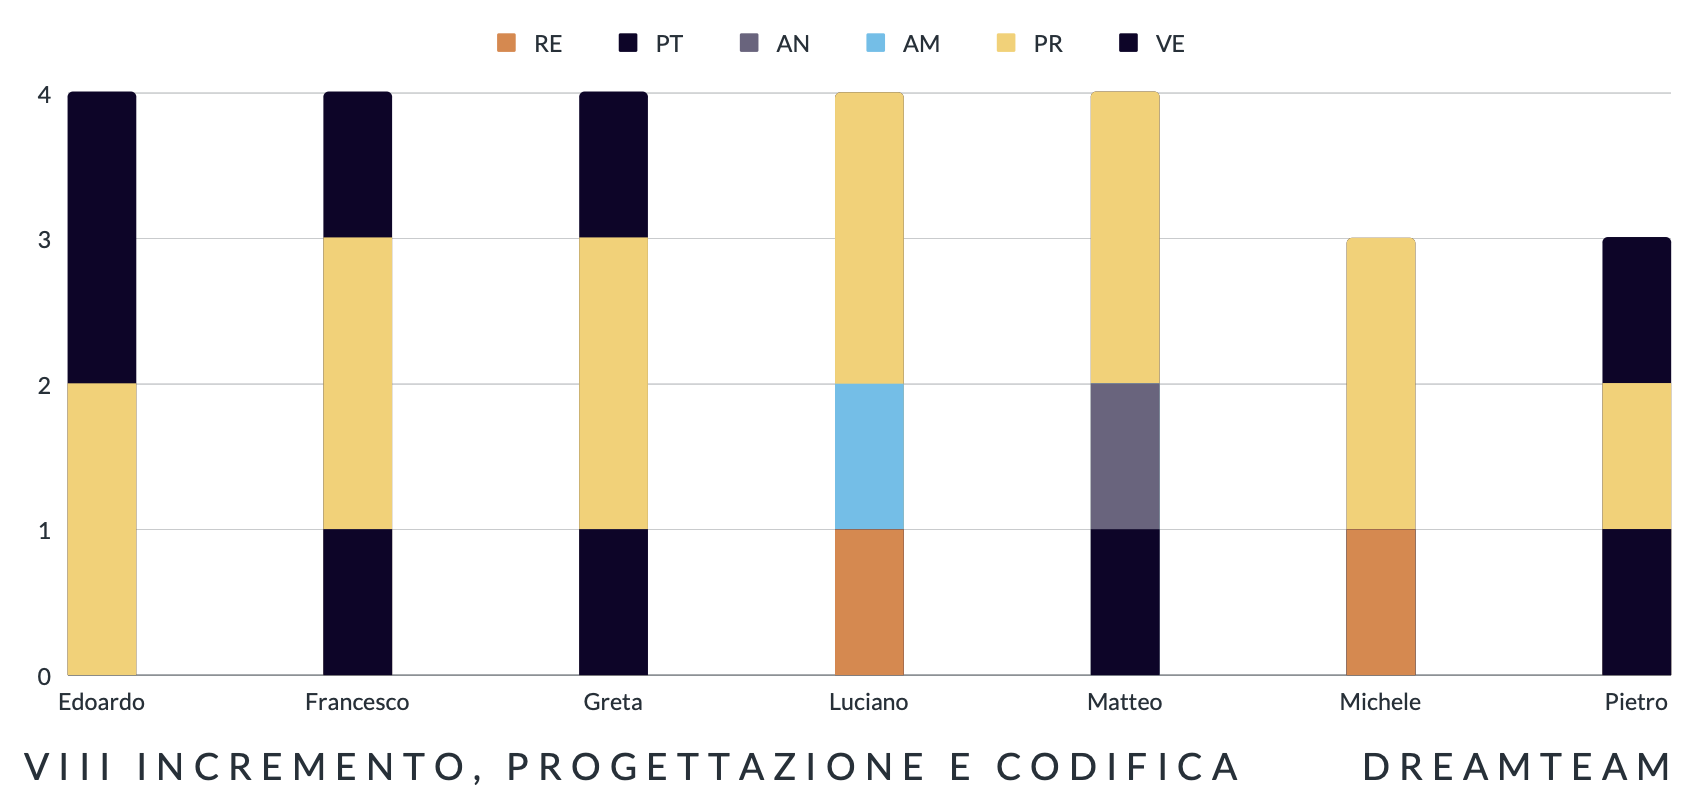
\includegraphics[scale=0.55]{Sezioni/SezioniPreventivo/grafici/Preventivo_progettazione_VIII.png}
\caption{Istogramma della ripartizione delle ore nel VIII incremento di Progettazione e Codifica}
\end{figure}

\subsubsubsection{Prospetto economico}
La seguente tabella rappresenta le ore totali dedicate ad ogni ruolo e il costo in euro:

\begin{table}[H]
\begin{center}
\rowcolors{2}{gray!25}{white}
\renewcommand{\arraystretch}{1.5}
\begin{tabular}{ m{0.3\textwidth}<{\centering}  m{0.2\textwidth}<{\centering} m{0.2\textwidth}<{\centering}}
	\rowcolor{darkblue}
	\textcolor{white}{\textbf{Ruolo}}&\textcolor{white}{\textbf{Totale ore}}&\textcolor{white}{\textbf{Costo totale (\euro)}}\\ 

	Responsabile  & 2 & 60 \\	
	
	Progettista & 4 & 80 \\
	
	Analista & 1 & 25 \\

	Amministratore & 1 & 25 \\
	
	Programmatore & 13 & 195 \\
	
	Verificatore & 6 & 90 \\
	
	\textbf{Totale} & 27 & 475 \\
	
\end{tabular}
\caption{Prospetto dei costi per ruolo nel VIII incremento di Progettazione e Codifica}
\end{center}
\end{table}

La tabella può essere rappresentata anche in forma visiva dal seguente aerogramma:
\begin{figure}[H]
\centering
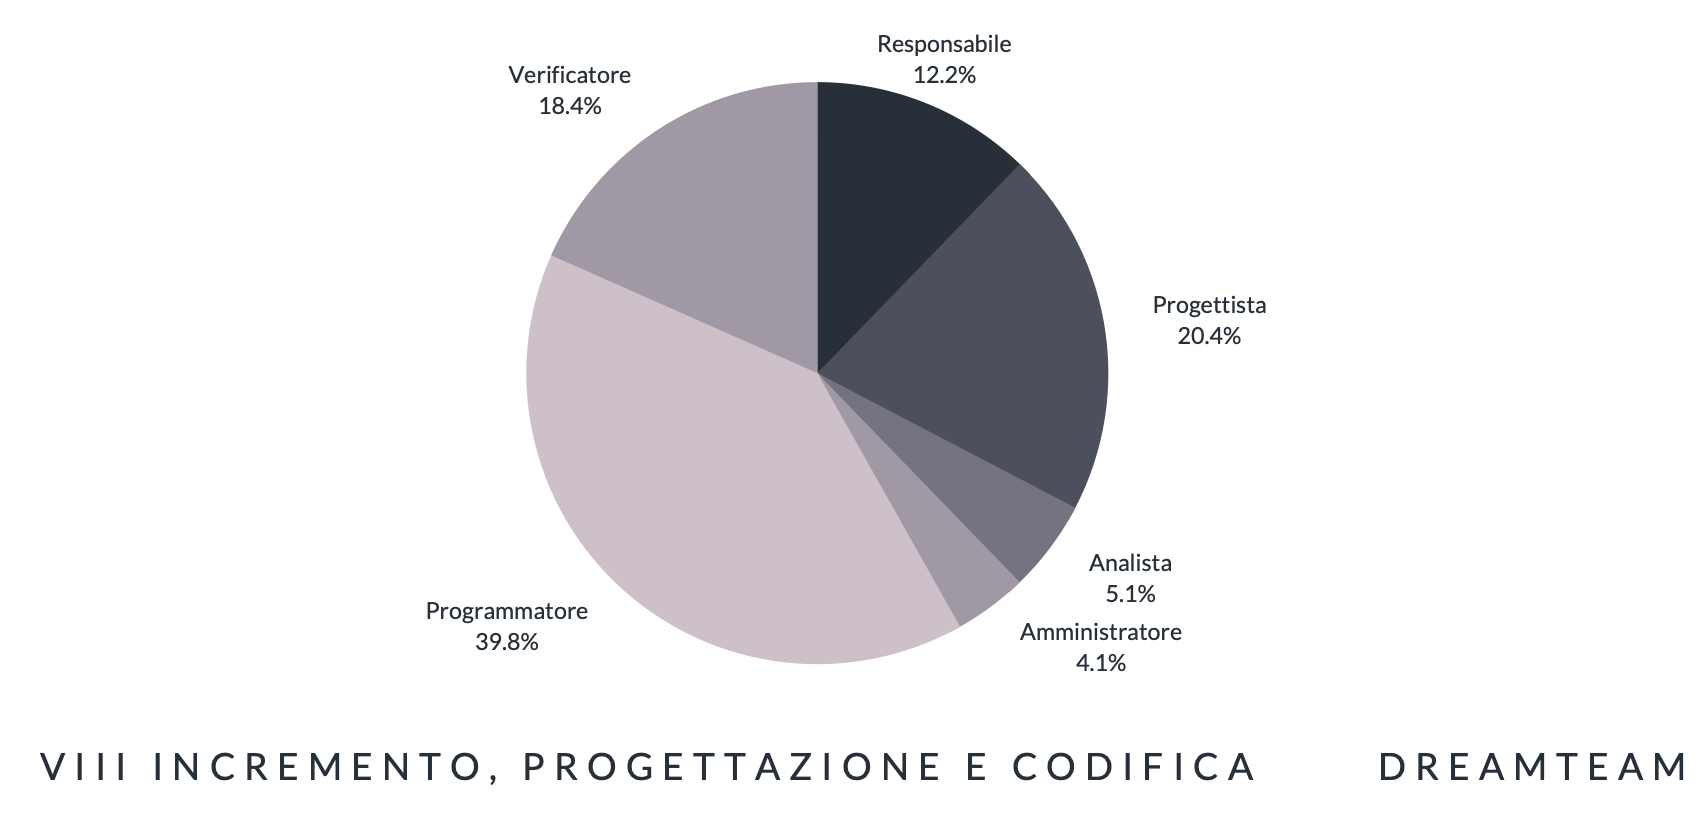
\includegraphics[scale=0.55]{Sezioni/SezioniPreventivo/grafici/Preventivo_torta_progettazione_VIII.png}
\caption{Grafico a torta della ripartizione per ruolo delle ore durante il VIII incremento di Progettazione e Codifica}
\end{figure}

\pagebreak


\subsubsection{Fase complessiva}
\subsubsubsection{Prospetto orario}
La seguente tabella rappresenta la distribuzione oraria per ogni componente del gruppo nella fase di progettazione e codifica:
\begin{table}[H]
\begin{center}
\rowcolors{2}{gray!25}{white}
\renewcommand{\arraystretch}{1.25}
\begin{tabular}{ m{0.20\textwidth}<{\centering}  m{0.06\textwidth}<{\centering} m{0.06\textwidth}<{\centering} m{0.06\textwidth}<{\centering}  m{0.06\textwidth}<{\centering}  m{0.06\textwidth}<{\centering}  m{0.06\textwidth}<{\centering}  m{0.20\textwidth}<{\centering}   }
	\rowcolor{darkblue}
	\textcolor{white}{\textbf{Componente}} &\textcolor{white}{\textbf{Re}}&\textcolor{white}{\textbf{Pt}}&\textcolor{white}{\textbf{An}}&\textcolor{white}{\textbf{Am}}&\textcolor{white}{\textbf{Pr}}&\textcolor{white}{\textbf{Ve}}&\textcolor{white}{\textbf{Ore complessive}}\\ 
	Edoardo Pavan & 2 & 13 & 0 & 7 & 22 & 10 & 54 \\	
	
	Francesco Protopapa & 2 & 8 & 0 & 1 & 20 & 6 & 37 \\

	Greta Cavedon & 3 & 7 & 0 & 0 & 16 & 10 & 36 \\
	
	Luciano Wu & 5 & 10 & 0 & 4 & 16 & 6 & 41 \\
	
	Matteo Basso & 0 & 9 & 10 & 0 & 15 & 7 & 41 \\
	
	Michele Gatto &  6 & 8 & 0 & 0 & 20 & 5 & 39 \\
	
	Pietro Villatora & 0 & 8 & 0 & 2 & 31 & 6 & 47 \\
	
	\textbf{Ore totali ruolo} & 18 & 63 & 10 & 14 & 140 & 50 & 295\\

\end{tabular}
\caption{Distribuzione oraria per ogni componente nella fase di Progettazione e Codifica}
\end{center}
\end{table}

La tabella può essere rappresentata anche in forma visiva dal seguente grafico:
\begin{figure}[H]
\centering
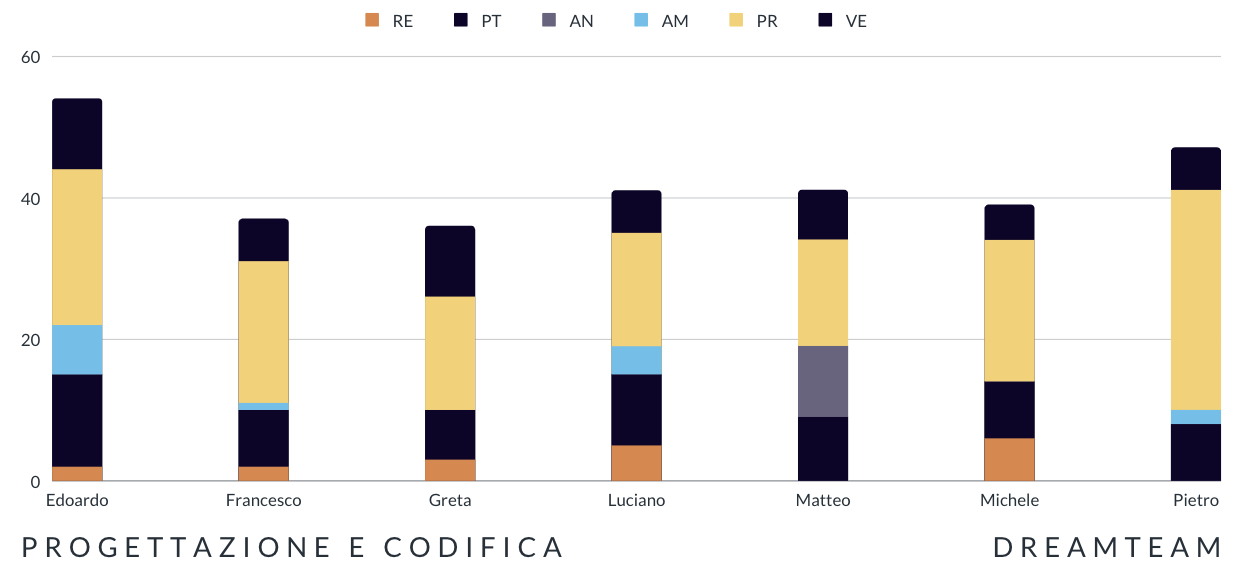
\includegraphics[scale=0.65]{Sezioni/SezioniPreventivo/grafici/Progettazione_codifica.png}
\caption{Istogramma della ripartizione delle ore nella fase di Progettazione e Codifica}
\end{figure}

\subsubsubsection{Prospetto economico}
La seguente tabella rappresenta le ore totali dedicate ad ogni ruolo e il costo in euro:

\begin{table}[H]
\begin{center}
\rowcolors{2}{gray!25}{white}
\renewcommand{\arraystretch}{1.5}
\begin{tabular}{ m{0.3\textwidth}<{\centering}  m{0.2\textwidth}<{\centering} m{0.2\textwidth}<{\centering}}
	\rowcolor{darkblue}
	\textcolor{white}{\textbf{Ruolo}}&\textcolor{white}{\textbf{Totale ore}}&\textcolor{white}{\textbf{Costo totale (\euro)}}\\ 

	Responsabile  & 18 & 540 \\	
	
	Progettista & 63 & 1575 \\
	
	Analista & 10 & 250 \\

	Amministratore & 14 & 280 \\
	
	Programmatore & 140 & 2100 \\
	
	Verificatore & 50 & 750 \\
	
	\textbf{Totale} & 295 & 5495 \\
	
\end{tabular}
\caption{Prospetto dei costi per ruolo nella fase di Progettazione e Codifica}
\end{center}
\end{table}

La tabella può essere rappresentata anche in forma visiva dal seguente aerogramma:
\begin{figure}[H]
\centering
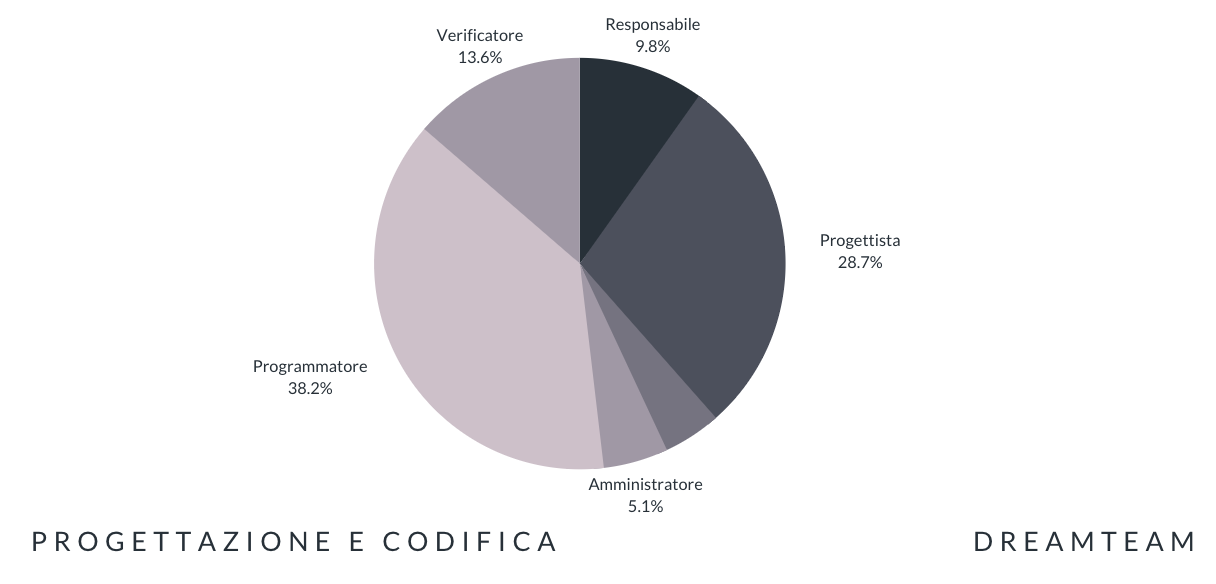
\includegraphics[scale=0.65]{Sezioni/SezioniPreventivo/grafici/Progettazione_costi.png}
\caption{Grafico a torta della ripartizione per ruolo delle ore durante la fase di Progettazione e Codifica}
\end{figure}



